\documentclass[conference]{IEEEtran}
% Based on the IEEE conference LaTeX template dated June 27, 2024.
% Do not add geometry, titlesec, caption, or font packages: IEEEtran controls
% the page dimensions, typography, headings, captions, and column layout.

\usepackage{cite}
\usepackage{amsmath,amssymb,amsfonts}
\usepackage{graphicx}
\usepackage{textcomp}
\usepackage{xcolor}
\usepackage{balance}

\def\BibTeX{{\rm B\kern-.05em{\sc i\kern-.025em b}\kern-.08em
    T\kern-.1667em\lower.7ex\hbox{E}\kern-.125emX}}

\graphicspath{{figures/}}

\begin{document}

\title{A Reproducible BB84 Quantum Key Distribution Simulator with
Illustrative Finite-Key Analysis}

\author{\IEEEauthorblockN{Lam Thanh Dat}
\IEEEauthorblockA{\textit{Department of Telecommunications}\\
\textit{Faculty of Electrical and Electronics Engineering}\\
\textit{Ho Chi Minh City University of Technology (HCMUT), VNU-HCM}\\
Ho Chi Minh City, Vietnam}
}

\maketitle

\begin{abstract}
Quantum key distribution exploits measurement disturbance to reveal
eavesdropping during secret-key establishment. This paper presents a
reproducible Python simulator of the Bennett--Brassard 1984 protocol under
detection loss, intrinsic bit errors, intercept--resend attacks, heuristic
information leakage, and finite data blocks. The implementation separates an
asymptotic secret-fraction model from an illustrative finite-size correction
and provides validated command-line and graphical interfaces, deterministic
parameter sweeps, and automated tests. In a reference run with one hundred
thousand emitted signal slots, an ideal link produced zero quantum bit error
rate, whereas a full intercept--resend attack produced a rate of 24.79 percent
and eliminated the estimated secret-key budget. For an error-correction
inefficiency of 1.15, the implemented asymptotic equation gives a critical
error rate of 9.88 percent. Finite-size sweeps show that the gap from the
asymptotic estimate decreases with increasing block size. The simulator is
intended for education, model verification, and sensitivity analysis; it is
not a composable security proof or a deployable quantum key distribution
system.
\end{abstract}

\begin{IEEEkeywords}
BB84, finite-key analysis, Monte Carlo simulation, quantum communication,
quantum key distribution, reproducible research.
\end{IEEEkeywords}

\section{Introduction}

The Bennett--Brassard 1984 (BB84) protocol encodes classical information in
nonorthogonal quantum states and uses public basis reconciliation to form a
shared sifted key \cite{bennett1984}. An eavesdropper who measures unknown
states generally disturbs them, allowing the legitimate users to estimate the
quantum bit error rate (QBER) and abort when the disturbance is excessive.
Security proofs relate the observed bit and phase errors to an extractable
secret-key length under explicit protocol assumptions \cite{shor2000}.

Educational implementations can reproduce this qualitative behavior, but
their numerical output is meaningful only when the channel abstraction,
postprocessing budget, and finite-size assumptions are stated precisely.
In particular, a Monte Carlo confidence interval quantifies variation across
simulated trials; it is not a cryptographic security bound. Likewise, an
estimated secret length is not equivalent to executing error correction,
verification, authentication, and privacy amplification.

This work standardizes a project-scale BB84 simulator and makes three
contributions. First, it separates detection loss, intrinsic bit errors, and
intercept--resend disturbance instead of combining them in one ambiguous
efficiency parameter. Second, it implements deterministic experiments,
machine-readable outputs, input validation, and automated tests. Third, it
audits the equations used by the source project and corrects the critical QBER
associated with the selected error-correction inefficiency. The contribution
is therefore reproducible modeling and software engineering rather than a new
QKD security proof.

\section{System Model}

\subsection{Signal preparation, detection, and sifting}

For each of \(N\) emitted signal slots, Alice independently samples a bit and
one of the \(Z\) and \(X\) bases. Bob independently selects a measurement
basis. A detected event is retained only when the bases agree. Two event
detection models are exposed:
\begin{equation}
p_{\mathrm{det}} =
\begin{cases}
\min(\mu\eta,1), & \text{linear approximation},\\
1-\exp(-\mu\eta), & \text{Poisson approximation},
\end{cases}
\label{eq:detection}
\end{equation}
where \(\mu\) is the mean photon number or normalized source intensity and
\(\eta\) is the receiver-efficiency factor. The first expression preserves
compatibility with the source project. The second is the at-least-one-event
probability of the simplified Poisson model. Neither expression includes dark
counts or detector dead time.

The parameter \(F_b\) denotes intrinsic bit fidelity, so the independent
channel-flip probability is \(1-F_b\). Eve attacks each signal independently
with probability \(p_{\mathrm{atk}}\), measures it in a random BB84 basis, and
resends the result. In an otherwise ideal link, Eve selects the wrong basis
with probability one half and Bob then obtains a wrong bit with probability
one half. The expected attack-induced QBER is consequently
\begin{equation}
\mathbb{E}[Q_{\mathrm{atk}}]=\frac{1}{4}p_{\mathrm{atk}}.
\label{eq:attack}
\end{equation}

\subsection{Asymptotic secret-fraction estimate}

For \(0\leq x\leq1\), the binary entropy is
\begin{equation}
h_2(x)=-x\log_2x-(1-x)\log_2(1-x),
\label{eq:entropy}
\end{equation}
with the endpoint values defined by continuity. Let \(Q\) be the measured
QBER, \(f_{\mathrm{EC}}\geq1\) the error-correction inefficiency, and
\(\lambda\) a heuristic fractional leakage penalty. The simulator estimates
the asymptotic secret fraction per retained sifted bit as
\begin{equation}
r_{\infty}
=
\left[1-(1+f_{\mathrm{EC}})h_2(Q)\right]^+(1-\lambda),
\label{eq:asymptotic}
\end{equation}
where \([x]^+=\max(x,0)\). Equation~\eqref{eq:asymptotic} is an information
budget; no reconciliation code or privacy-amplification hash is executed.
For \(f_{\mathrm{EC}}=1.15\), the zero-key condition
\((1+f_{\mathrm{EC}})h_2(Q_{\mathrm{crit}})=1\) gives
\(Q_{\mathrm{crit}}=0.09878\), or approximately \(9.88\%\).

\subsection{Illustrative finite-size estimate}

For \(n\) sifted bits, the finite-size module expands the observed QBER using a
normal-quantile margin:
\begin{align}
\delta &=
z_{1-\varepsilon_{\mathrm{sec}}/2}
\sqrt{\frac{\max\{Q(1-Q),10^{-12}\}}{n}},
\label{eq:margin}\\
Q_{\mathrm{ph}}^{U} &= \min\!\left(Q+\delta,\frac{1}{2}\right),
\label{eq:phase}
\end{align}
where \(\varepsilon_{\mathrm{sec}}\) is the configured secrecy parameter.
The provisional bit budget is
\begin{align}
\ell &=
n\!\left[1-f_{\mathrm{EC}}h_2(Q)
-h_2\!\left(Q_{\mathrm{ph}}^{U}\right)\right]-\Delta_{\mathrm{sec}},
\label{eq:finite}\\
\Delta_{\mathrm{sec}}
&=2\log_2\!\frac{1}{\varepsilon_{\mathrm{sec}}}
+\log_2\!\frac{2}{\varepsilon_{\mathrm{cor}}},
\label{eq:overhead}
\end{align}
and the reported length is
\(\ell_{\mathrm{fin}}=\lfloor(1-\lambda)\max(0,\ell)\rfloor\).
Here, this construction is used only for sensitivity analysis. Composable
finite-key security requires a protocol-specific treatment with rigorous
random-sampling bounds, single-photon parameter estimation, and complete
allocation of failure probabilities \cite{tomamichel2012}.

\section{Implementation and Reproducibility}

The software is organized as an installable Python package. Immutable parameter
and result records provide explicit interfaces for the asymptotic and
finite-size models. Validation rejects probabilities outside the unit interval,
negative source intensity, nonpositive block size, and
\(f_{\mathrm{EC}}<1\). A command-line interface supports single-run,
finite-size, and threshold calculations; a desktop interface calls the same
validated model functions.

The reproduction script creates reference JSON, comma-separated tables, and
vector and raster figures. Independent deterministic seeds are assigned to
each sweep point and repetition. The unit-test suite covers entropy endpoints,
detection models, attack behavior, threshold calculation, finite-size trends,
reproducibility, invalid inputs, result synchronization, and command-line
output. The numerical
configurations used in the paper are summarized in Table~\ref{tab:settings}.

\begin{table}[t]
\caption{Configurations for the Reported Sweeps}
\label{tab:settings}
\centering
\footnotesize
\setlength{\tabcolsep}{3pt}
\begin{tabular}{lcc}
\hline
\textbf{Parameter} & \textbf{Attack sweep} & \textbf{Finite-size sweep}\\
\hline
Emitted slots \(N\) & \(2\times10^5\) & \(10^4\) to \(3\times10^6\)\\
Mean photon number \(\mu\) & 1.0 & 0.4\\
Intrinsic bit fidelity \(F_b\) & 1.0 & 0.98\\
Receiver efficiency \(\eta\) & 1.0 & 0.9\\
Attack probability \(p_{\mathrm{atk}}\) & 0 to 1 & 0\\
Repetitions per point & 8 & 5\\
\(\varepsilon_{\mathrm{sec}},\varepsilon_{\mathrm{cor}}\) & --- & \(10^{-9},10^{-9}\)\\
\hline
\end{tabular}
\end{table}

\section{Numerical Results}

\subsection{Reference scenarios}

Table~\ref{tab:scenarios} reports deterministic runs with \(10^5\) emitted
signal slots and seed 2025. The ideal, intercept--resend, and intrinsic-error
cases use \(\mu=\eta=1\), \(f_{\mathrm{EC}}=1.15\), no heuristic leakage, and
192 disclosed-bit deductions after QBER evaluation.

\begin{table}[t]
\caption{Deterministic Reference Scenarios}
\label{tab:scenarios}
\centering
\footnotesize
\setlength{\tabcolsep}{3.5pt}
\begin{tabular}{lrrr}
\hline
\textbf{Scenario} & \(\boldsymbol{Q}\) & \(\boldsymbol{r_{\infty}}\) &
\textbf{Key bits}\\
\hline
Ideal baseline & 0.0000 & 1.0000 & 50001\\
Full intercept--resend & 0.2479 & 0.0000 & 0\\
Five-percent intrinsic error & 0.0513 & 0.3722 & 18611\\
Above-threshold error & 0.1361 & 0.0000 & 0\\
\hline
\end{tabular}
\end{table}

The full intercept--resend case gives \(Q=0.2479\), consistent with
\eqref{eq:attack}. The five-percent intrinsic-error case retains a positive
budget, whereas the above-threshold case is clipped to zero by
\eqref{eq:asymptotic}. The calculated threshold of \(9.88\%\) corrects the
\(10.3\%\) value stated in the source report for the same equation and
\(f_{\mathrm{EC}}\).

\begin{figure*}[t]
\centering
\begin{minipage}[t]{0.485\textwidth}
\centering
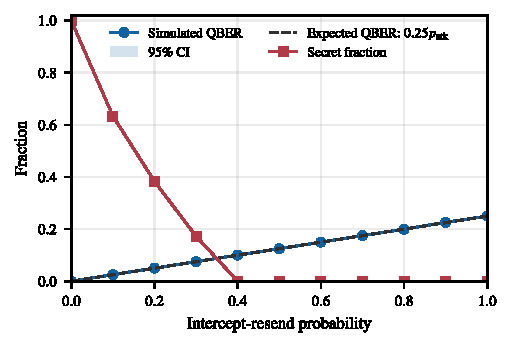
\includegraphics[width=\linewidth]{bb84_intercept_resend_sweep.pdf}
\centerline{\footnotesize (a)}
\end{minipage}
\hfill
\begin{minipage}[t]{0.485\textwidth}
\centering
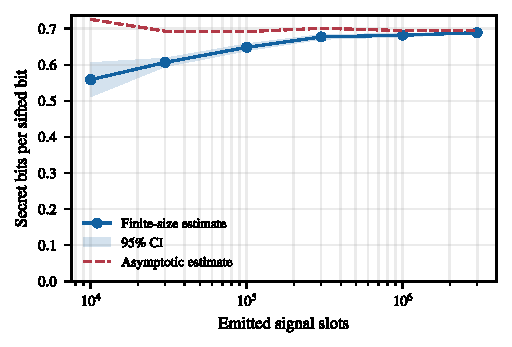
\includegraphics[width=\linewidth]{bb84_finite_key_scaling.pdf}
\centerline{\footnotesize (b)}
\end{minipage}
\caption{Reproducible Monte Carlo sweeps. (a) QBER and the asymptotic secret
fraction versus intercept--resend probability. (b) Illustrative finite-size
secret fraction versus emitted signal slots. The shaded bands are 95\% normal
confidence intervals for the simulated mean; they are neither experimental
uncertainty intervals nor cryptographic security bounds.}
\label{fig:sweeps}
\end{figure*}

\subsection{Attack sweep}

As shown in Fig.~\ref{fig:sweeps}(a), the mean QBER follows
\(0.25p_{\mathrm{atk}}\) over the tested range. At full attack, the eight-run
mean is 0.24979. The estimated secret fraction decreases nonlinearly because
QBER enters the entropy function. It remains 0.1728 at
\(p_{\mathrm{atk}}=0.3\), where the mean QBER is 0.0751, and becomes zero at
\(p_{\mathrm{atk}}=0.4\), where the mean QBER is 0.1003. The transition agrees
with the calculated critical QBER.

\subsection{Finite-size trend}

The finite-size sweep in Fig.~\ref{fig:sweeps}(b) uses the Poisson detection
model and the settings in Table~\ref{tab:settings}. At \(N=10^4\), the mean
finite-size fraction is 0.5588, compared with an asymptotic estimate of 0.7261.
At \(N=3\times10^6\), the corresponding values are 0.6890 and 0.6963. The
shrinking gap is consistent with the \(n^{-1/2}\) statistical margin in
\eqref{eq:margin}. These results also show that a universal zero-key cutoff
below \(10^5\) emitted slots is not supported by this parameter set.

\section{Discussion and Limitations}

The experiments reproduce the principal qualitative behavior expected from
the implemented abstraction. Intercept--resend disturbance raises QBER
approximately linearly, the entropy-based secret budget collapses after the
model-specific threshold, and finite data impose a penalty that decreases as
the block grows. Detection loss reduces the number of detected and sifted
events; in the present model it does not itself introduce errors.

The numerical outputs must not be interpreted as certified secure-key rates.
QBER is evaluated over the entire sifted sequence before a fixed disclosure
count is deducted, rather than being estimated from the disclosed sample. The
deducted positions are selected through a seed-reproducible random mask for
retained-bit bookkeeping, but sampling uncertainty is not propagated. The
simulator accounts for error-correction and privacy-amplification leakage but
does not execute either algorithm. It also
omits authentication, dark counts, afterpulsing, dead time, timing jitter,
source fluctuations, detector-efficiency mismatch, and correlated noise.

The source model does not estimate the yield or error rate of the single-photon
component. Its heuristic leakage penalty is not a decoy-state calculation
\cite{lo2005,ma2005}. The code also omits the detector-side protection of
measurement-device-independent QKD. The normal approximation in
\eqref{eq:margin} is not a substitute for a tight composable finite-key proof.
These restrictions are material: removing them requires a new protocol model,
not merely additional simulation trials \cite{scarani2009,xu2020}.

\section{Conclusion}

A report-scale BB84 program has been converted into a reproducible research
repository and documented with explicit mathematical and security boundaries.
The simulator validates the expected one-quarter QBER under full
intercept--resend, identifies a \(9.88\%\) critical QBER for the implemented
model with \(f_{\mathrm{EC}}=1.15\), and demonstrates convergence of an
illustrative finite-size estimate toward its asymptotic counterpart. Future
work should implement decoy-state single-photon bounds, rigorous concentration
inequalities, authenticated classical communication, error-correction codes,
and universal-hash privacy amplification before physical secure-key-rate
claims are considered.

\section*{Acknowledgment}

The author thanks Prof. Le Tien Thuong for supervision. OpenAI's ChatGPT,
including Codex, was used to assist with English-language editing, refactoring
of the accompanying Python implementation, preparation of software tests, and
initial drafting of the abstract and explanatory prose in Sections III--VI.
The author retains responsibility for the technical content and final approval.

\balance
\begin{thebibliography}{00}

\bibitem{bennett1984}
C. H. Bennett and G. Brassard, ``Quantum cryptography: Public key distribution
and coin tossing,'' in \emph{Proc. IEEE Int. Conf. Computers, Systems and
Signal Processing}, Bangalore, India, 1984, pp. 175--179.

\bibitem{shor2000}
P. W. Shor and J. Preskill, ``Simple proof of security of the BB84 quantum key
distribution protocol,'' \emph{Phys. Rev. Lett.}, vol. 85, no. 2,
pp. 441--444, Jul. 2000, doi: 10.1103/PhysRevLett.85.441.

\bibitem{tomamichel2012}
M. Tomamichel, C. C. W. Lim, N. Gisin, and R. Renner, ``Tight finite-key
analysis for quantum cryptography,'' \emph{Nat. Commun.}, vol. 3,
Art. no. 634, Jan. 2012, doi: 10.1038/ncomms1631.

\bibitem{lo2005}
H.-K. Lo, X. Ma, and K. Chen, ``Decoy state quantum key distribution,''
\emph{Phys. Rev. Lett.}, vol. 94, no. 23, Art. no. 230504, Jun. 2005,
doi: 10.1103/PhysRevLett.94.230504.

\bibitem{ma2005}
X. Ma, B. Qi, Y. Zhao, and H.-K. Lo, ``Practical decoy state for quantum key
distribution,'' \emph{Phys. Rev. A}, vol. 72, no. 1, Art. no. 012326,
Jul. 2005, doi: 10.1103/PhysRevA.72.012326.

\bibitem{scarani2009}
V. Scarani, H. Bechmann-Pasquinucci, N. J. Cerf, M. Du\v{s}ek,
N. L\"utkenhaus, and M. Peev, ``The security of practical quantum key
distribution,'' \emph{Rev. Mod. Phys.}, vol. 81, no. 3, pp. 1301--1350,
Sep. 2009, doi: 10.1103/RevModPhys.81.1301.

\bibitem{xu2020}
F. Xu, X. Ma, Q. Zhang, H.-K. Lo, and J.-W. Pan, ``Secure quantum key
distribution with realistic devices,'' \emph{Rev. Mod. Phys.}, vol. 92,
no. 2, Art. no. 025002, May 2020,
doi: 10.1103/RevModPhys.92.025002.

\end{thebibliography}

\end{document}
